\documentclass[12pt,]{book}
\usepackage{lmodern}
\usepackage{amssymb,amsmath}
\usepackage{ifxetex,ifluatex}
\usepackage{fixltx2e} % provides \textsubscript
\ifnum 0\ifxetex 1\fi\ifluatex 1\fi=0 % if pdftex
  \usepackage[T1]{fontenc}
  \usepackage[utf8]{inputenc}
\else % if luatex or xelatex
  \ifxetex
    \usepackage{mathspec}
  \else
    \usepackage{fontspec}
  \fi
  \defaultfontfeatures{Ligatures=TeX,Scale=MatchLowercase}
\fi
% use upquote if available, for straight quotes in verbatim environments
\IfFileExists{upquote.sty}{\usepackage{upquote}}{}
% use microtype if available
\IfFileExists{microtype.sty}{%
\usepackage{microtype}
\UseMicrotypeSet[protrusion]{basicmath} % disable protrusion for tt fonts
}{}
\usepackage[margin=1in]{geometry}
\usepackage{hyperref}
\hypersetup{unicode=true,
            pdftitle={Statistical Methods for Research II},
            pdfauthor={Shizhe Chen},
            pdfborder={0 0 0},
            breaklinks=true}
\urlstyle{same}  % don't use monospace font for urls
\usepackage{natbib}
\bibliographystyle{apalike}
\usepackage{color}
\usepackage{fancyvrb}
\newcommand{\VerbBar}{|}
\newcommand{\VERB}{\Verb[commandchars=\\\{\}]}
\DefineVerbatimEnvironment{Highlighting}{Verbatim}{commandchars=\\\{\}}
% Add ',fontsize=\small' for more characters per line
\usepackage{framed}
\definecolor{shadecolor}{RGB}{248,248,248}
\newenvironment{Shaded}{\begin{snugshade}}{\end{snugshade}}
\newcommand{\KeywordTok}[1]{\textcolor[rgb]{0.13,0.29,0.53}{\textbf{#1}}}
\newcommand{\DataTypeTok}[1]{\textcolor[rgb]{0.13,0.29,0.53}{#1}}
\newcommand{\DecValTok}[1]{\textcolor[rgb]{0.00,0.00,0.81}{#1}}
\newcommand{\BaseNTok}[1]{\textcolor[rgb]{0.00,0.00,0.81}{#1}}
\newcommand{\FloatTok}[1]{\textcolor[rgb]{0.00,0.00,0.81}{#1}}
\newcommand{\ConstantTok}[1]{\textcolor[rgb]{0.00,0.00,0.00}{#1}}
\newcommand{\CharTok}[1]{\textcolor[rgb]{0.31,0.60,0.02}{#1}}
\newcommand{\SpecialCharTok}[1]{\textcolor[rgb]{0.00,0.00,0.00}{#1}}
\newcommand{\StringTok}[1]{\textcolor[rgb]{0.31,0.60,0.02}{#1}}
\newcommand{\VerbatimStringTok}[1]{\textcolor[rgb]{0.31,0.60,0.02}{#1}}
\newcommand{\SpecialStringTok}[1]{\textcolor[rgb]{0.31,0.60,0.02}{#1}}
\newcommand{\ImportTok}[1]{#1}
\newcommand{\CommentTok}[1]{\textcolor[rgb]{0.56,0.35,0.01}{\textit{#1}}}
\newcommand{\DocumentationTok}[1]{\textcolor[rgb]{0.56,0.35,0.01}{\textbf{\textit{#1}}}}
\newcommand{\AnnotationTok}[1]{\textcolor[rgb]{0.56,0.35,0.01}{\textbf{\textit{#1}}}}
\newcommand{\CommentVarTok}[1]{\textcolor[rgb]{0.56,0.35,0.01}{\textbf{\textit{#1}}}}
\newcommand{\OtherTok}[1]{\textcolor[rgb]{0.56,0.35,0.01}{#1}}
\newcommand{\FunctionTok}[1]{\textcolor[rgb]{0.00,0.00,0.00}{#1}}
\newcommand{\VariableTok}[1]{\textcolor[rgb]{0.00,0.00,0.00}{#1}}
\newcommand{\ControlFlowTok}[1]{\textcolor[rgb]{0.13,0.29,0.53}{\textbf{#1}}}
\newcommand{\OperatorTok}[1]{\textcolor[rgb]{0.81,0.36,0.00}{\textbf{#1}}}
\newcommand{\BuiltInTok}[1]{#1}
\newcommand{\ExtensionTok}[1]{#1}
\newcommand{\PreprocessorTok}[1]{\textcolor[rgb]{0.56,0.35,0.01}{\textit{#1}}}
\newcommand{\AttributeTok}[1]{\textcolor[rgb]{0.77,0.63,0.00}{#1}}
\newcommand{\RegionMarkerTok}[1]{#1}
\newcommand{\InformationTok}[1]{\textcolor[rgb]{0.56,0.35,0.01}{\textbf{\textit{#1}}}}
\newcommand{\WarningTok}[1]{\textcolor[rgb]{0.56,0.35,0.01}{\textbf{\textit{#1}}}}
\newcommand{\AlertTok}[1]{\textcolor[rgb]{0.94,0.16,0.16}{#1}}
\newcommand{\ErrorTok}[1]{\textcolor[rgb]{0.64,0.00,0.00}{\textbf{#1}}}
\newcommand{\NormalTok}[1]{#1}
\usepackage{longtable,booktabs}
\usepackage{graphicx,grffile}
\makeatletter
\def\maxwidth{\ifdim\Gin@nat@width>\linewidth\linewidth\else\Gin@nat@width\fi}
\def\maxheight{\ifdim\Gin@nat@height>\textheight\textheight\else\Gin@nat@height\fi}
\makeatother
% Scale images if necessary, so that they will not overflow the page
% margins by default, and it is still possible to overwrite the defaults
% using explicit options in \includegraphics[width, height, ...]{}
\setkeys{Gin}{width=\maxwidth,height=\maxheight,keepaspectratio}
\IfFileExists{parskip.sty}{%
\usepackage{parskip}
}{% else
\setlength{\parindent}{0pt}
\setlength{\parskip}{6pt plus 2pt minus 1pt}
}
\setlength{\emergencystretch}{3em}  % prevent overfull lines
\providecommand{\tightlist}{%
  \setlength{\itemsep}{0pt}\setlength{\parskip}{0pt}}
\setcounter{secnumdepth}{5}
% Redefines (sub)paragraphs to behave more like sections
\ifx\paragraph\undefined\else
\let\oldparagraph\paragraph
\renewcommand{\paragraph}[1]{\oldparagraph{#1}\mbox{}}
\fi
\ifx\subparagraph\undefined\else
\let\oldsubparagraph\subparagraph
\renewcommand{\subparagraph}[1]{\oldsubparagraph{#1}\mbox{}}
\fi

%%% Use protect on footnotes to avoid problems with footnotes in titles
\let\rmarkdownfootnote\footnote%
\def\footnote{\protect\rmarkdownfootnote}

%%% Change title format to be more compact
\usepackage{titling}

% Create subtitle command for use in maketitle
\providecommand{\subtitle}[1]{
  \posttitle{
    \begin{center}\large#1\end{center}
    }
}

\setlength{\droptitle}{-2em}

  \title{Statistical Methods for Research II}
    \pretitle{\vspace{\droptitle}\centering\huge}
  \posttitle{\par}
    \author{Shizhe Chen}
    \preauthor{\centering\large\emph}
  \postauthor{\par}
      \predate{\centering\large\emph}
  \postdate{\par}
    \date{2020-01-09}

\usepackage{booktabs}
\usepackage{amsthm}
\makeatletter
\def\thm@space@setup{%
  \thm@preskip=8pt plus 2pt minus 4pt
  \thm@postskip=\thm@preskip
}
\makeatother

\begin{document}
\maketitle

{
\setcounter{tocdepth}{1}
\tableofcontents
}
\chapter*{Preface}\label{pre}
\addcontentsline{toc}{chapter}{Preface}

This file contains code and comments in STA 207. Many materials in this
document are adapted from lectures by Professors Prabir Burman, Peng
Ding, and \href{https://imai.fas.harvard.edu/teaching/index.html}{Kosuke
Imai}.

\chapter{Causal Inference}\label{ch:causal}

\section{Association and Causality}\label{association-and-causality}

\section{Potential Outcomes}\label{potential-outcomes}

\begin{itemize}
\tightlist
\item
  Definition of potential outcomes
\item
  Properties of potential outcomes
\item
  Key assumptions in this notation
\item
  Immutable characteristics
\end{itemize}

\section{Experiments v.s. Observational
Studies}\label{experiments-v.s.-observational-studies}

\begin{itemize}
\tightlist
\item
  Advantages of randomized experiments
\item
  Reasons for observational studies
\end{itemize}

\section{Learning Objectives}\label{learning-objectives}

\begin{itemize}
\tightlist
\item
  Students are able to distinguish association and causality.
\item
  Students gain basic familiarity with the potential outcome framework.
\item
  Students are able to recognize the importance of experiment designs.
\end{itemize}

\chapter{One-way ANOVA}\label{ch:anovaI}

\section{Simple randomized
experiments}\label{simple-randomized-experiments}

\begin{itemize}
\tightlist
\item
  Motivation and real world applications of randomized experiments.
\item
  Sampling schemes of a simple randomized experiment.
\item
  Question of interest, null hypotheses, and their causal
  interpretation.
\item
  Intuition of hypothesis testing.
\item
  Practical concerns in the design of experiments.
\end{itemize}

\section{One-way ANOVA}\label{one-way-anova}

\subsection{A motivating example: the Spock
trial}\label{a-motivating-example-the-spock-trial}

In 1968 Dr.~Benjamin Spock was tried in Boston for conspiring against
the government for helping young men to escape the military draft. He
was convicted by the Boston federal court, but the judgement was
overturned by the Court of Appeals in 1969 for many reasons, one of
which was cited as the bias of the presiding judge Francis Ford.
Dr.~Spock, a pediatrician, was very famous for his books on rearing of
children, and thus was widely admired by women. As a matter of fact, the
jury in Spock trial has no women. Note that jury panels, though randomly
selected, should reflect the demographics. In any particular trial,
there may not be any woman on the jury, but it is worthwhile to examine
if the jury panels of Judge Ford had fewer women than other judges in
Boston in few months before the trial. Data are available for jury
panels for 7, but we investigate the data for only 4 judges including
Judge Ford.

\begin{Shaded}
\begin{Highlighting}[]
\NormalTok{Spock <-}\StringTok{ }\KeywordTok{read.csv}\NormalTok{(}\DataTypeTok{file=}\StringTok{"./data/SpockTrial.csv"}\NormalTok{, }\DataTypeTok{header=}\OtherTok{TRUE}\NormalTok{, }\DataTypeTok{sep=}\StringTok{","}\NormalTok{)}
\NormalTok{Spock}\OperatorTok{$}\NormalTok{Judge<-}\KeywordTok{as.factor}\NormalTok{(Spock}\OperatorTok{$}\NormalTok{Judge);}
\CommentTok{# Box plot with jittered points (from stackoverflow: https://stackoverflow.com/questions/23675735/how-to-add-boxplots-to-scatterplot-with-jitter)}
\KeywordTok{boxplot}\NormalTok{(perc.women}\OperatorTok{~}\NormalTok{Judge,}\DataTypeTok{data=}\NormalTok{Spock)}
\KeywordTok{stripchart}\NormalTok{(perc.women}\OperatorTok{~}\NormalTok{Judge, }\DataTypeTok{vertical =} \OtherTok{TRUE}\NormalTok{, }\DataTypeTok{data =}\NormalTok{ Spock, }
    \DataTypeTok{method =} \StringTok{"jitter"}\NormalTok{, }\DataTypeTok{add =} \OtherTok{TRUE}\NormalTok{, }\DataTypeTok{pch =} \DecValTok{20}\NormalTok{, }\DataTypeTok{col =} \StringTok{'blue'}\NormalTok{)}
\end{Highlighting}
\end{Shaded}

\begin{figure}

{\centering 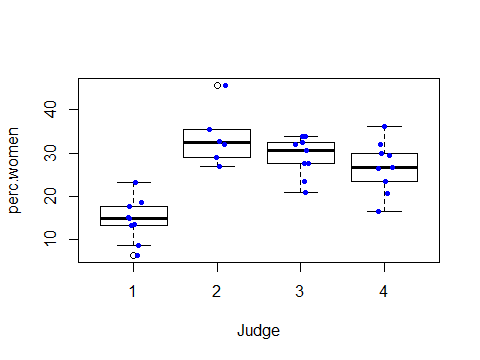
\includegraphics[width=0.8\linewidth]{STA207_bookdown_files/figure-latex/fig-anovaI-1} 

}

\caption{Box plot with jittered data points for the Spock trial data.}\label{fig:fig-anovaI}
\end{figure}

\subsection{ANOVA model}\label{anova-model}

\begin{itemize}
\tightlist
\item
  Cell means model
\item
  Estimators of the means
\item
  Decomposition of sum of squares
\item
  Some basic properties
\end{itemize}

In the Spock trial data, we can use \texttt{aov()} to fit a one-way
ANOVA model.

\begin{Shaded}
\begin{Highlighting}[]
\NormalTok{anova.fit<-}\StringTok{ }\KeywordTok{aov}\NormalTok{(perc.women}\OperatorTok{~}\NormalTok{Judge,}\DataTypeTok{data=}\NormalTok{Spock)}
\KeywordTok{summary}\NormalTok{(anova.fit)}
\end{Highlighting}
\end{Shaded}

\begin{verbatim}
##             Df Sum Sq Mean Sq F value  Pr(>F)    
## Judge        3   1591     530    17.6 1.1e-06 ***
## Residuals   29    874      30                    
## ---
## Signif. codes:  0 '***' 0.001 '**' 0.01 '*' 0.05 '.' 0.1 ' ' 1
\end{verbatim}

We can obtain the following.

\begin{itemize}
\tightlist
\item
  \(n_1=\) 9, \(n_2=\) 6, \(n_3=\) 9, \(n_4=\) 9, and
  \(n_T=n_1+n_2+n_3+n_4=\) 33.
\item
  \(\bar{Y}_{1,\cdot}=\) 14.62, \(\bar{Y}_{2,\cdot}=\) 33.62,
  \(\bar{Y}_{3,\cdot}=\) 29.1, and \(\bar{Y}_{4,\cdot}=\) 26.8.
\item
  \(SSE=\) 873.52, \(df=\) 29, and \(MSE=\) 30.12.
\item
  \(SSTO=\) 2464.8, \(df=\) 32.
\item
  \(SSTR=\) 1591.28, \(df=\) 3, and \(MSTR=\) 530.43.
\end{itemize}

\subsection{Statistical inference}\label{statistical-inference}

\begin{itemize}
\tightlist
\item
  Null hypothesis
\item
  The F-test
\item
  Testing a linear combination

  \begin{itemize}
  \tightlist
  \item
    Estimation
  \item
    Hypothesis testing
  \end{itemize}
\item
  (Simultaneous) confidence intervals
\end{itemize}

To test the null hypothesis \(H_0: \mu_1=\mu_2=\mu_3=\mu_4\) against the
alternative \(H_1:\) not all \(\mu_i\)'s are equal. We can calculate the
F-statistics \(F^*=\frac{MSTR}{MSE}=\) , \(F(0.95;3,29)=\) 2.93. We can
thus reject the null hypothesis at the chosen significance level
\(0.05\).

Consider the quantity \(L=\mu_1-(\mu_2+\mu_3+\mu4)/3\). We can calculate
that \(\hat{L}=\) -15.22, and \(s^2(\hat{L})=\) 4.65. Moreover, since
\(t(1-0.01/2;n_T-r)=\) 2.76 a \(99\%\) confidence interval for \(L\) is
(-21.16, -9.27).

To test the hypothesis \(H_0: L=0\) against \(H_1: L \neq 0\). We can
calculate the t-statistics \(t^*=\hat{L}/s(\hat{L})=\) -7.06. We can
calculate the quantile of the t-distribution as before to finish the
test.

Next we demonstrate how to contruct the simultaneous confidence
intervals for all pairwise difference. The code will construct
confidence intervals for two pairs, but leave you to finish the rest.

\begin{Shaded}
\begin{Highlighting}[]
\CommentTok{# Create vectors for the first two linear combinations }
\NormalTok{comb.mat<-}\KeywordTok{matrix}\NormalTok{(}\DecValTok{0}\NormalTok{,}\DataTypeTok{nrow=}\DecValTok{2}\NormalTok{,}\DataTypeTok{ncol=}\DecValTok{4}\NormalTok{)}
\NormalTok{comb.mat[}\DecValTok{1}\NormalTok{,]=}\KeywordTok{c}\NormalTok{(}\DecValTok{1}\NormalTok{,}\OperatorTok{-}\DecValTok{1}\NormalTok{,}\DecValTok{0}\NormalTok{,}\DecValTok{0}\NormalTok{);comb.mat[}\DecValTok{2}\NormalTok{,]=}\KeywordTok{c}\NormalTok{(}\DecValTok{1}\NormalTok{,}\DecValTok{0}\NormalTok{,}\OperatorTok{-}\DecValTok{1}\NormalTok{,}\DecValTok{0}\NormalTok{);}

\CommentTok{# Obtain the estimates }
\NormalTok{diff =}\StringTok{ }\KeywordTok{numeric}\NormalTok{(}\KeywordTok{dim}\NormalTok{(comb.mat)[}\DecValTok{1}\NormalTok{]);}
\NormalTok{diff.sd=diff;}
\NormalTok{mean.tmp=anova.fit}\OperatorTok{$}\NormalTok{coefficients;mean.tmp[}\DecValTok{1}\NormalTok{]=}\DecValTok{0}\NormalTok{;}
\NormalTok{ns=}\KeywordTok{as.numeric}\NormalTok{(}\KeywordTok{table}\NormalTok{(Spock}\OperatorTok{$}\NormalTok{Judge));}
\ControlFlowTok{for}\NormalTok{(i }\ControlFlowTok{in} \DecValTok{1}\OperatorTok{:}\KeywordTok{length}\NormalTok{(diff))\{}
\NormalTok{  diff[i]=}\KeywordTok{sum}\NormalTok{(comb.mat[i,]}\OperatorTok{*}\NormalTok{mean.tmp);}
\NormalTok{  diff.sd[i]=}\KeywordTok{sqrt}\NormalTok{(}\KeywordTok{sum}\NormalTok{(comb.mat[i,]}\OperatorTok{^}\DecValTok{2}\OperatorTok{*}\NormalTok{ns));}
\NormalTok{\}}

\NormalTok{alpha=}\FloatTok{0.05}\NormalTok{;}

\CommentTok{# Bonferroni correction:}
\NormalTok{m=}\DecValTok{6}\NormalTok{; }\CommentTok{# for all pairwise differences, although we only show two here}
\NormalTok{B.stat=}\KeywordTok{qt}\NormalTok{(}\DecValTok{1}\OperatorTok{-}\NormalTok{alpha}\OperatorTok{/}\NormalTok{(}\DecValTok{2}\OperatorTok{*}\NormalTok{m),anova.fit}\OperatorTok{$}\NormalTok{df.residual);}

\CommentTok{# Tukey-Kramer }
\NormalTok{T.stat=}\KeywordTok{qtukey}\NormalTok{(}\DecValTok{1}\OperatorTok{-}\NormalTok{alpha, }\DataTypeTok{nmeans=}\KeywordTok{length}\NormalTok{(anova.fit}\OperatorTok{$}\NormalTok{coefficients), }\DataTypeTok{df=}\NormalTok{anova.fit}\OperatorTok{$}\NormalTok{df.residual)}\OperatorTok{/}\KeywordTok{sqrt}\NormalTok{(}\DecValTok{2}\NormalTok{);}

\CommentTok{# Scheffe }
\NormalTok{S.stat=}\KeywordTok{sqrt}\NormalTok{( (}\KeywordTok{length}\NormalTok{(anova.fit}\OperatorTok{$}\NormalTok{coefficients)}\OperatorTok{-}\DecValTok{1}\NormalTok{)}\OperatorTok{*}\KeywordTok{qf}\NormalTok{(}\DecValTok{1}\OperatorTok{-}\NormalTok{alpha,}\KeywordTok{length}\NormalTok{(anova.fit}\OperatorTok{$}\NormalTok{coefficients)}\OperatorTok{-}\DecValTok{1}\NormalTok{,anova.fit}\OperatorTok{$}\NormalTok{df.residual))}

\NormalTok{table.stats=}\KeywordTok{matrix}\NormalTok{(}\DecValTok{0}\NormalTok{,}\DecValTok{1}\NormalTok{,}\DecValTok{3}\NormalTok{);}
\NormalTok{table.stats[}\DecValTok{1}\NormalTok{,]=}\KeywordTok{c}\NormalTok{(B.stat,T.stat,S.stat);}
\KeywordTok{colnames}\NormalTok{(table.stats)=}\KeywordTok{c}\NormalTok{(}\StringTok{'Bonferroni'}\NormalTok{, }\StringTok{'Tukey'}\NormalTok{, }\StringTok{'Scheffe'}\NormalTok{)}
\NormalTok{table.stats}
\end{Highlighting}
\end{Shaded}

\begin{verbatim}
##      Bonferroni Tukey Scheffe
## [1,]        2.8   2.7       3
\end{verbatim}

\begin{Shaded}
\begin{Highlighting}[]
\CommentTok{# Then, we can construct the confidence intervals as, e.g.,}
\NormalTok{CI.bonferroni =}\KeywordTok{matrix}\NormalTok{(}\DecValTok{0}\NormalTok{,}\DataTypeTok{nrow=}\DecValTok{2}\NormalTok{,}\DataTypeTok{ncol=}\DecValTok{2}\NormalTok{);}
\ControlFlowTok{for}\NormalTok{(i }\ControlFlowTok{in} \DecValTok{1}\OperatorTok{:}\KeywordTok{length}\NormalTok{(diff))\{}
\NormalTok{  CI.bonferroni[i,]=diff[i]}\OperatorTok{+}\KeywordTok{c}\NormalTok{(}\DecValTok{1}\NormalTok{,}\OperatorTok{-}\DecValTok{1}\NormalTok{)}\OperatorTok{*}\NormalTok{B.stat}\OperatorTok{*}\NormalTok{diff.sd[i];}
\NormalTok{\}}
\end{Highlighting}
\end{Shaded}

\subsection{Alternative forms of the ANOVA
model}\label{alternative-forms-of-the-anova-model}

\begin{itemize}
\tightlist
\item
  Factor-effect model
\item
  Regression model
\end{itemize}

The default of ANOVA in \texttt{R} set weights proportional to the
sample size in each cell. You can supply the \texttt{weights} to the
\texttt{aov()} function to force equal weights.

\begin{Shaded}
\begin{Highlighting}[]
\CommentTok{# Weights proportional to sample sizes }
\KeywordTok{print}\NormalTok{(}\KeywordTok{model.tables}\NormalTok{(anova.fit,}\StringTok{"effects"}\NormalTok{))}
\end{Highlighting}
\end{Shaded}

\begin{verbatim}
## Tables of effects
## 
##  Judge 
##          1     2     3     4
##     -10.72 8.271 3.755 1.455
## rep   9.00 6.000 9.000 9.000
\end{verbatim}

\section{Model diagnostics}\label{model-diagnostics}

\begin{itemize}
\tightlist
\item
  Possible departures
\item
  Diagnostics with residuals
\item
  Graphical methods
\item
  Formal tests

  \begin{itemize}
  \tightlist
  \item
    Hartley test
  \item
    Bartlett test
  \item
    Levene test
  \end{itemize}
\item
  Remedial measures

  \begin{itemize}
  \tightlist
  \item
    Weighted least squares
  \item
    Nonparametric tests based on ranks: rank test, Kruskal-Wallis test
  \item
    Box-Cox transformation
  \end{itemize}
\end{itemize}

All diagnostics start with the residuals.

\begin{Shaded}
\begin{Highlighting}[]
\CommentTok{# Obtain the residuals from the ANOVA fit}
\NormalTok{residuals=anova.fit}\OperatorTok{$}\NormalTok{residuals;}
\KeywordTok{hist}\NormalTok{(residuals)}
\end{Highlighting}
\end{Shaded}

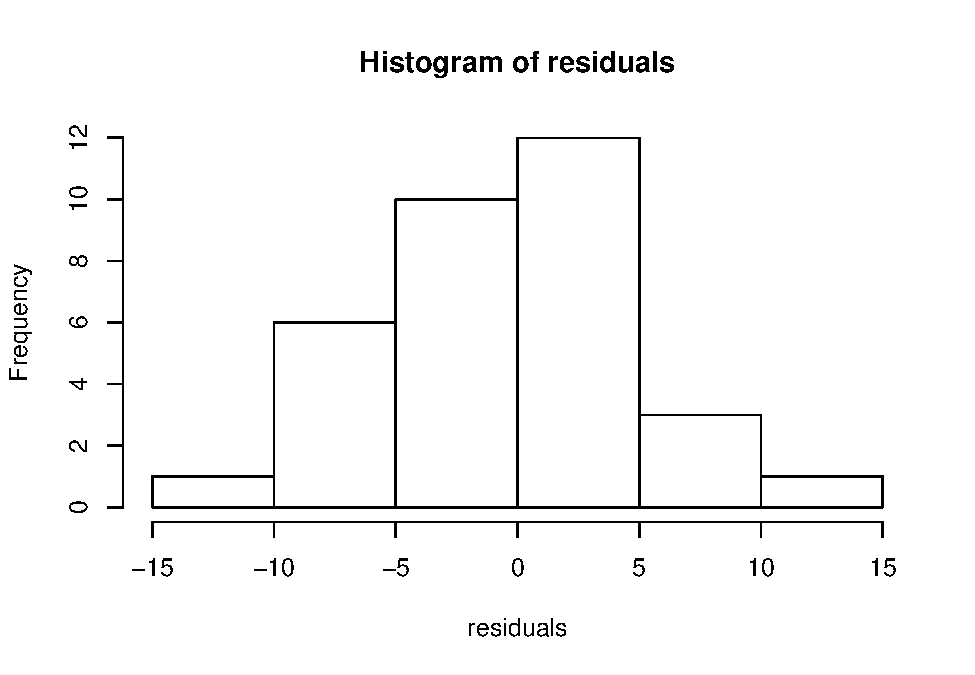
\includegraphics{STA207_bookdown_files/figure-latex/unnamed-chunk-6-1.pdf}

\begin{Shaded}
\begin{Highlighting}[]
\CommentTok{# Semistudentized residuals}
\NormalTok{residuals.semistd=anova.fit}\OperatorTok{$}\NormalTok{residuals}\OperatorTok{/}\KeywordTok{sqrt}\NormalTok{(mse);}
\KeywordTok{hist}\NormalTok{(residuals.semistd)}
\end{Highlighting}
\end{Shaded}

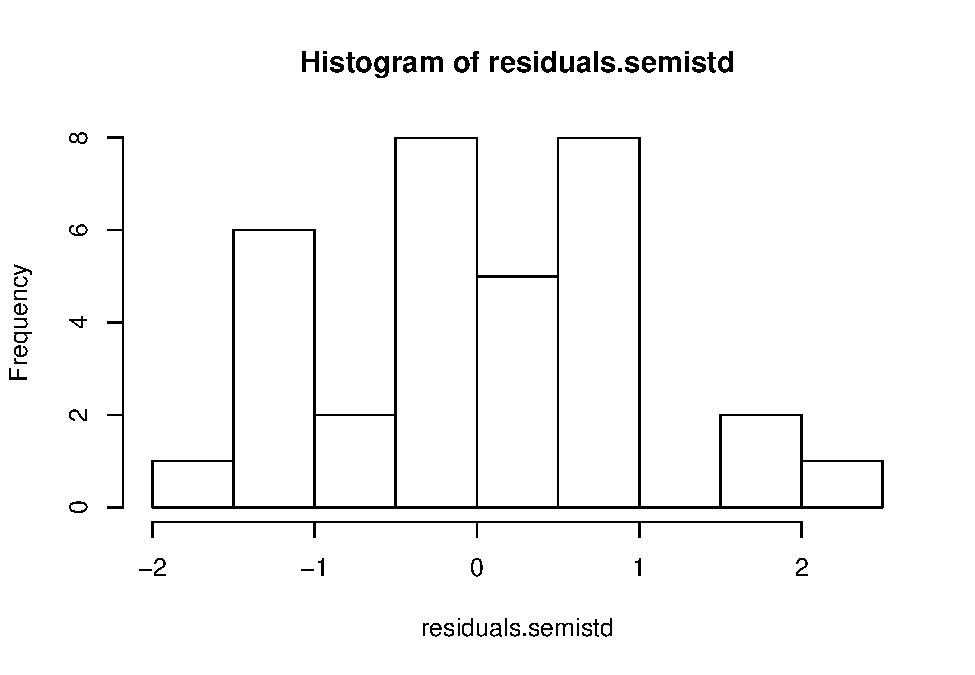
\includegraphics{STA207_bookdown_files/figure-latex/unnamed-chunk-6-2.pdf}

\begin{Shaded}
\begin{Highlighting}[]
\CommentTok{# Studentized residuals }
\NormalTok{weights=}\DecValTok{1}\OperatorTok{-}\DecValTok{1}\OperatorTok{/}\NormalTok{ns[}\KeywordTok{as.numeric}\NormalTok{(Spock}\OperatorTok{$}\NormalTok{Judge)];}
\NormalTok{residuals.std=anova.fit}\OperatorTok{$}\NormalTok{residuals}\OperatorTok{/}\KeywordTok{sqrt}\NormalTok{(mse)}\OperatorTok{/}\KeywordTok{sqrt}\NormalTok{(weights);}
\KeywordTok{hist}\NormalTok{(residuals.std)}
\end{Highlighting}
\end{Shaded}

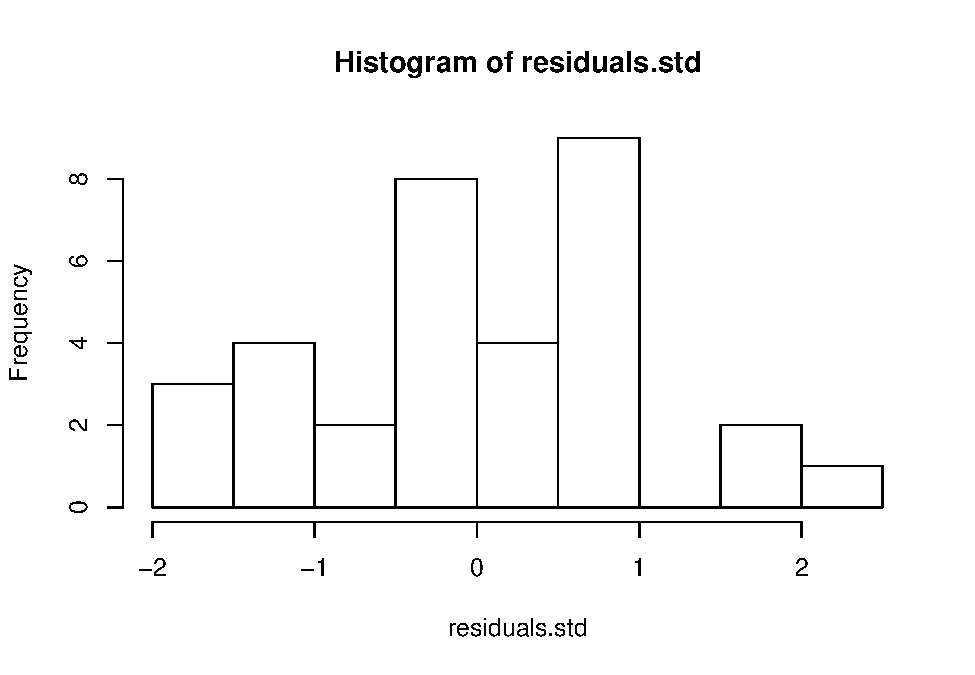
\includegraphics{STA207_bookdown_files/figure-latex/unnamed-chunk-6-3.pdf}

\begin{Shaded}
\begin{Highlighting}[]
\CommentTok{# Plot the residuals (or the other two versions) against fitted values }
\KeywordTok{plot}\NormalTok{(residuals}\OperatorTok{~}\NormalTok{anova.fit}\OperatorTok{$}\NormalTok{fitted.values,}\DataTypeTok{type=}\StringTok{'p'}\NormalTok{,}\DataTypeTok{pch=}\DecValTok{16}\NormalTok{,}\DataTypeTok{cex=}\FloatTok{1.5}\NormalTok{,}\DataTypeTok{xlab=}\StringTok{"Fitted values"}\NormalTok{,}\DataTypeTok{ylab=}\StringTok{"Residuals"}\NormalTok{)}
\end{Highlighting}
\end{Shaded}

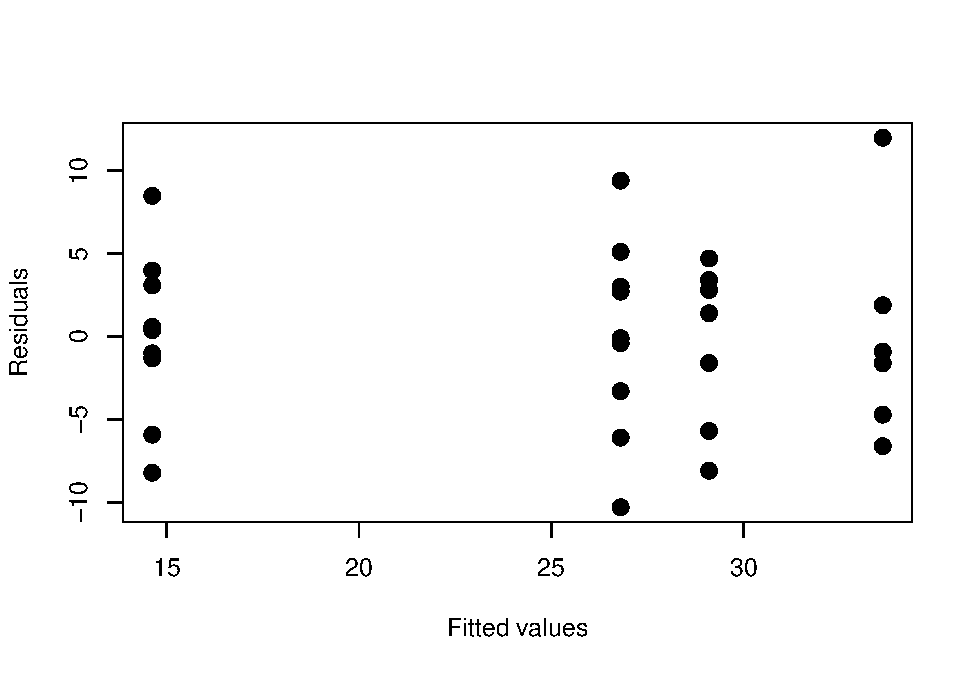
\includegraphics{STA207_bookdown_files/figure-latex/unnamed-chunk-7-1.pdf}

\begin{Shaded}
\begin{Highlighting}[]
\CommentTok{# Plot the residual against certain orders}
\CommentTok{# No clear orders make sense in the Spock trial data }

\CommentTok{# Stem-leaf plot  (or use histogram, or qq-plot )}
\KeywordTok{stem}\NormalTok{(residuals)}
\end{Highlighting}
\end{Shaded}

\begin{verbatim}
## 
##   The decimal point is at the |
## 
##   -10 | 3
##    -8 | 21
##    -6 | 61
##    -4 | 977
##    -2 | 3
##    -0 | 66630941
##     0 | 4649
##     2 | 78014
##     4 | 0771
##     6 | 
##     8 | 54
##    10 | 
##    12 | 0
\end{verbatim}

\begin{Shaded}
\begin{Highlighting}[]
\KeywordTok{qqnorm}\NormalTok{(residuals);}\KeywordTok{qqline}\NormalTok{(residuals)}
\end{Highlighting}
\end{Shaded}

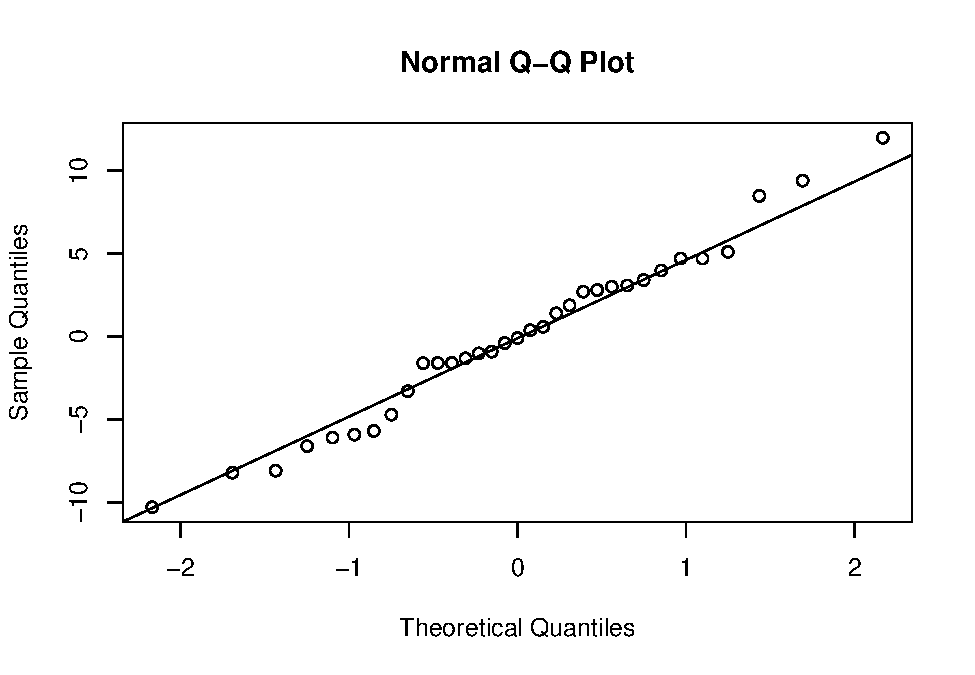
\includegraphics{STA207_bookdown_files/figure-latex/unnamed-chunk-7-2.pdf}

\begin{Shaded}
\begin{Highlighting}[]
\CommentTok{# Plot residuals against missing variables }
\CommentTok{# Not applicable on Spock trial data }
\end{Highlighting}
\end{Shaded}

We now turn to formal tests of the equality of variances.

\begin{Shaded}
\begin{Highlighting}[]
\CommentTok{# Calculate the variances for each group:}
\NormalTok{(}\DataTypeTok{vars =} \KeywordTok{tapply}\NormalTok{(Spock}\OperatorTok{$}\NormalTok{perc.women,Spock}\OperatorTok{$}\NormalTok{Judge,var))}
\end{Highlighting}
\end{Shaded}

\begin{verbatim}
##  1  2  3  4 
## 25 43 21 36
\end{verbatim}

\begin{Shaded}
\begin{Highlighting}[]
\NormalTok{alpha=}\FloatTok{0.05}\NormalTok{;}

\CommentTok{# Hartley test:}
\NormalTok{H.stat=}\KeywordTok{max}\NormalTok{(vars)}\OperatorTok{/}\KeywordTok{min}\NormalTok{(vars);}
\KeywordTok{library}\NormalTok{(SuppDists) }\CommentTok{# The distribution is in this package}
\CommentTok{# Both df and k only take integers:}
\KeywordTok{qmaxFratio}\NormalTok{(}\DecValTok{1}\OperatorTok{-}\NormalTok{alpha,}\DataTypeTok{df=}\KeywordTok{floor}\NormalTok{(}\KeywordTok{sum}\NormalTok{(ns)}\OperatorTok{/}\KeywordTok{length}\NormalTok{(ns)}\OperatorTok{-}\DecValTok{1}\NormalTok{),}\DataTypeTok{k=}\KeywordTok{length}\NormalTok{(ns))}
\end{Highlighting}
\end{Shaded}

\begin{verbatim}
## [1] 8.4
\end{verbatim}

\begin{Shaded}
\begin{Highlighting}[]
\KeywordTok{qmaxFratio}\NormalTok{(}\DecValTok{1}\OperatorTok{-}\NormalTok{alpha,}\DataTypeTok{df=}\KeywordTok{ceiling}\NormalTok{(}\KeywordTok{sum}\NormalTok{(ns)}\OperatorTok{/}\KeywordTok{length}\NormalTok{(ns)}\OperatorTok{-}\DecValTok{1}\NormalTok{),}\DataTypeTok{k=}\KeywordTok{length}\NormalTok{(ns))}
\end{Highlighting}
\end{Shaded}

\begin{verbatim}
## [1] 7.2
\end{verbatim}

\begin{Shaded}
\begin{Highlighting}[]
\CommentTok{# Bartlett test:}
\NormalTok{K.stat=}\StringTok{ }\NormalTok{(}\KeywordTok{sum}\NormalTok{(ns)}\OperatorTok{-}\KeywordTok{length}\NormalTok{(ns))}\OperatorTok{*}\KeywordTok{log}\NormalTok{(mse)}\OperatorTok{-}\KeywordTok{sum}\NormalTok{( (ns}\OperatorTok{-}\DecValTok{1}\NormalTok{)}\OperatorTok{*}\KeywordTok{log}\NormalTok{(vars) );}
\KeywordTok{qchisq}\NormalTok{(}\DecValTok{1}\OperatorTok{-}\NormalTok{alpha,}\DataTypeTok{df=}\KeywordTok{length}\NormalTok{(ns)}\OperatorTok{-}\DecValTok{1}\NormalTok{)}
\end{Highlighting}
\end{Shaded}

\begin{verbatim}
## [1] 7.8
\end{verbatim}

\begin{Shaded}
\begin{Highlighting}[]
\CommentTok{# Levene test:}
\NormalTok{Spock}\OperatorTok{$}\NormalTok{res.abs=}\KeywordTok{abs}\NormalTok{(anova.fit}\OperatorTok{$}\NormalTok{residuals);}
\KeywordTok{summary}\NormalTok{(}\KeywordTok{aov}\NormalTok{(res.abs}\OperatorTok{~}\NormalTok{Judge,}\DataTypeTok{data=}\NormalTok{Spock))}
\end{Highlighting}
\end{Shaded}

\begin{verbatim}
##             Df Sum Sq Mean Sq F value Pr(>F)
## Judge        3    5.6    1.88    0.17   0.91
## Residuals   29  314.7   10.85
\end{verbatim}

We leave weighted least squares for exercise. You can either calculate
it following the steps discussed in lecture, or use the \texttt{weights}
option in \texttt{lm()} and \texttt{aov()}.

We can conduct the nonparametric tests as follows.

\begin{Shaded}
\begin{Highlighting}[]
\CommentTok{# The rank test}
\NormalTok{Spock}\OperatorTok{$}\NormalTok{rank.perc=}\KeywordTok{rank}\NormalTok{(Spock}\OperatorTok{$}\NormalTok{perc.women)}
\KeywordTok{summary}\NormalTok{(}\KeywordTok{aov}\NormalTok{(rank.perc}\OperatorTok{~}\NormalTok{Judge,}\DataTypeTok{data=}\NormalTok{Spock))}
\end{Highlighting}
\end{Shaded}

\begin{verbatim}
##             Df Sum Sq Mean Sq F value  Pr(>F)    
## Judge        3   1846     615    15.6 3.1e-06 ***
## Residuals   29   1144      39                    
## ---
## Signif. codes:  0 '***' 0.001 '**' 0.01 '*' 0.05 '.' 0.1 ' ' 1
\end{verbatim}

\begin{Shaded}
\begin{Highlighting}[]
\CommentTok{# Krusal-Wallis test:}
\KeywordTok{kruskal.test}\NormalTok{(perc.women}\OperatorTok{~}\NormalTok{Judge,}\DataTypeTok{data=}\NormalTok{Spock)}
\end{Highlighting}
\end{Shaded}

\begin{verbatim}
## 
##  Kruskal-Wallis rank sum test
## 
## data:  perc.women by Judge
## Kruskal-Wallis chi-squared = 20, df = 3, p-value = 2e-04
\end{verbatim}

For Box-Cox transformation, use the \texttt{boxcox} in library
\texttt{MASS}.

\section{Learning Objectives}\label{learning-objectives-1}

\begin{itemize}
\tightlist
\item
  Students are able to write down a one-way ANOVA model given a new
  dataset.
\item
  Students understand the basic properties of one-way ANOVA models.
\item
  Students recognize the assumptions associated with each method.
\item
  Students can implement the aforemened tasks in \texttt{R}.
\item
  Students are comfortable reading \texttt{R} helpfiles related to
  one-way ANOVA.
\end{itemize}

\chapter{Two-way ANOVA}\label{ch:anovaII}

\section{Experiments with two (or more)
factors}\label{experiments-with-two-or-more-factors}

\begin{itemize}
\tightlist
\item
  Randomized experiments with two treatments
\item
  Stratified randomized Experiments (also known as randomized block
  design)

  \begin{itemize}
  \tightlist
  \item
    Auditor training data
  \item
    Project STAR
  \end{itemize}
\item
  Reasons for stratification: practical and statistical
\item
  Sampling scheme for a stratified randomized experiment
\item
  Question of interest, null hypotheses, and their causal
  interpretation.
\item
  Intuition of hypothesis testing.
\end{itemize}

Description of the auditor training data: There are three training
methods for the auditors and the response \(Y\) is a proficiency score
after the training are completed. Ideally we would like to compare the
three methods among those who are as similar as possible in their
educational background. How do we achieve this? One way is compare the
three different training methods among those whose time since graduation
from college are about the same. Suppose then we have ten such groups
(of three individuals each). Group 1 consists of those who graduated
recently, group 2 people graduated between one and two years ago, and
group 10 consists of those who graduated some time in the past (say, ten
years or more). Time since graduation is called the block (or a blocking
factor) and treatment is the training method.

\section{Two-way ANOVA}\label{two-way-anova}

\subsection{A motivating example: Hey fever relief data
set}\label{a-motivating-example-hey-fever-relief-data-set}

For the Hay Fever Relief example, 9 compounds for Hay Fever Relief are
made by varying levels of the two basic ingredients. Ingredient 1
(factor A) has \(a = 3\) levels: low \((i = 1)\), medium \((i = 2)\) and
high \((i = 3)\). Similarly, ingredient 2 (factor B) has \(b = 3\)
levels: low \((j = 1)\), medium \((j = 2)\) and high \((j = 3)\). A
total of 36 subjects (suffering from hay fever) are selected and each of
the 9 compounds are given to randomly selected \(n = 4\) individuals.

\subsection{A two-way ANOVA model}\label{a-two-way-anova-model}

\begin{itemize}
\tightlist
\item
  Cell mean model
\item
  Decomposition of the means, and their estimators
\item
  Additive models

  \begin{itemize}
  \tightlist
  \item
    Why additive models?
  \item
    Estimators of the means
  \end{itemize}
\item
  Decomposition of sum of squares, and their properties
\end{itemize}

\subsection{Statistical inference}\label{statistical-inference-1}

\begin{itemize}
\tightlist
\item
  F-statistics based on sums of squares
\item
  Hypothesis testing

  \begin{itemize}
  \tightlist
  \item
    Test for interaction effects
  \item
    Test for main effects
  \item
    Alternative test if interaction can be ignored (additive models)
  \end{itemize}
\item
  (Simultaneous) confidence intervals with and without interactions

  \begin{itemize}
  \tightlist
  \item
    Bonferroni
  \item
    Tukey
  \item
    Scheffe
  \end{itemize}
\end{itemize}

\subsection{Model diagnostics}\label{model-diagnostics-1}

\begin{itemize}
\tightlist
\item
  Similar to those for one-way ANOVA
\end{itemize}

\subsection{Strategy for data
analysis}\label{strategy-for-data-analysis}

Using the Hey Fever data as an example.

\begin{Shaded}
\begin{Highlighting}[]
\NormalTok{Hay <-}\StringTok{ }\KeywordTok{read.csv}\NormalTok{(}\DataTypeTok{file=}\StringTok{"./data/HayFever.csv"}\NormalTok{, }\DataTypeTok{header=}\OtherTok{TRUE}\NormalTok{, }\DataTypeTok{sep=}\StringTok{","}\NormalTok{)}

\CommentTok{# Use a slightly different visualization:}
\KeywordTok{pairs}\NormalTok{(Hay,}\DataTypeTok{pch=}\DecValTok{16}\NormalTok{,}\DataTypeTok{col=}\StringTok{'red'}\NormalTok{,}\DataTypeTok{cex=}\FloatTok{1.5}\NormalTok{)}
\end{Highlighting}
\end{Shaded}

\begin{figure}

{\centering 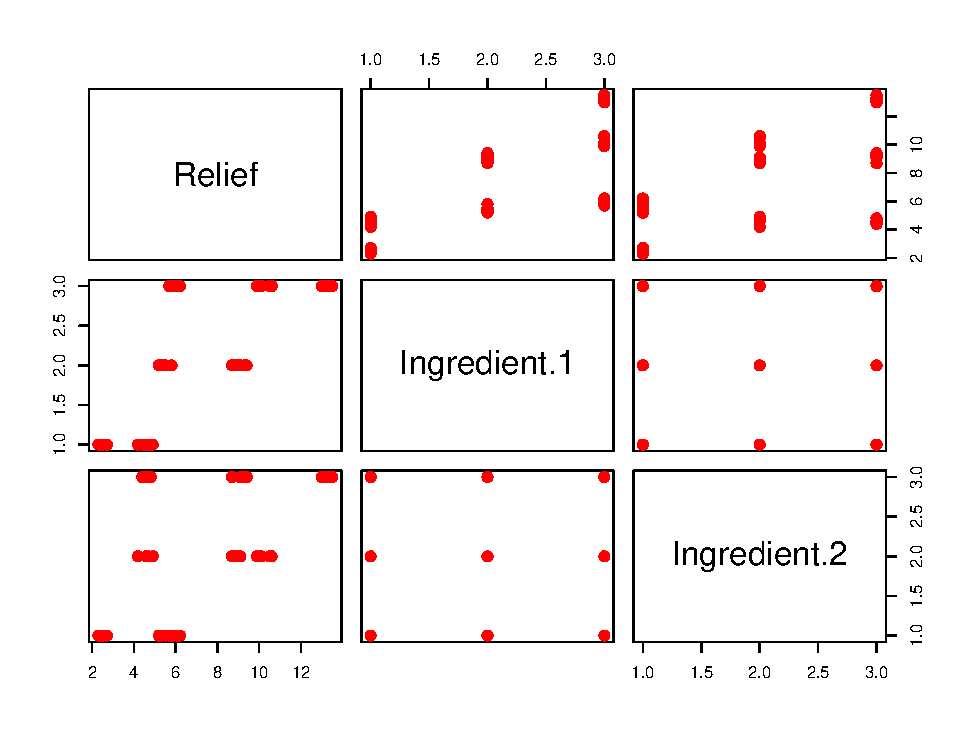
\includegraphics[width=0.8\linewidth]{STA207_bookdown_files/figure-latex/fig-anovaII-1} 

}

\caption{Box plot with jittered data points for the Spock trial data.}\label{fig:fig-anovaII1}
\end{figure}

\begin{Shaded}
\begin{Highlighting}[]
\CommentTok{# Or draw the interaction plot:}
\KeywordTok{interaction.plot}\NormalTok{(Hay}\OperatorTok{$}\NormalTok{Ingredient.}\DecValTok{1}\NormalTok{, Hay}\OperatorTok{$}\NormalTok{Ingredient.}\DecValTok{2}\NormalTok{, Hay}\OperatorTok{$}\NormalTok{Relief)}
\end{Highlighting}
\end{Shaded}

\begin{figure}

{\centering 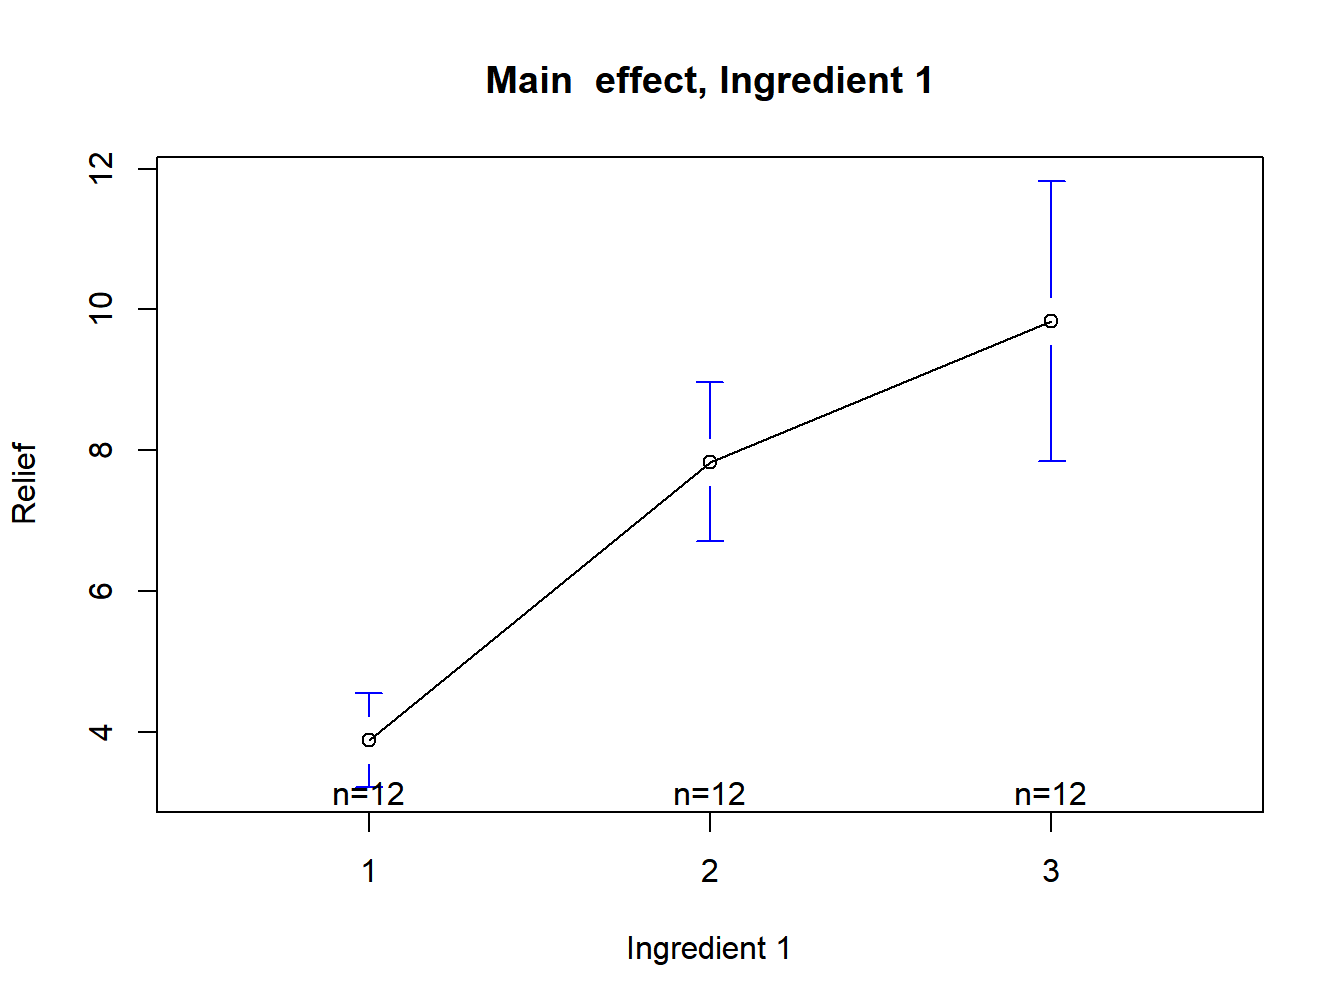
\includegraphics[width=0.8\linewidth]{STA207_bookdown_files/figure-latex/fig-anovaII-2} 

}

\caption{Box plot with jittered data points for the Spock trial data.}\label{fig:fig-anovaII2}
\end{figure}

Step 1. Test whether interaction effects are presented.

\begin{Shaded}
\begin{Highlighting}[]
\CommentTok{# We can use the regression form here}
\NormalTok{full_model=}\KeywordTok{lm}\NormalTok{(Relief}\OperatorTok{~}\KeywordTok{as.factor}\NormalTok{(Ingredient.}\DecValTok{1}\NormalTok{)}\OperatorTok{+}\KeywordTok{as.factor}\NormalTok{(Ingredient.}\DecValTok{2}\NormalTok{)}\OperatorTok{+}\KeywordTok{as.factor}\NormalTok{(Ingredient.}\DecValTok{1}\NormalTok{)}\OperatorTok{*}\KeywordTok{as.factor}\NormalTok{(Ingredient.}\DecValTok{2}\NormalTok{),}\DataTypeTok{data=}\NormalTok{Hay);}
\NormalTok{reduced_model=}\KeywordTok{lm}\NormalTok{(Relief}\OperatorTok{~}\KeywordTok{as.factor}\NormalTok{(Ingredient.}\DecValTok{1}\NormalTok{)}\OperatorTok{+}\KeywordTok{as.factor}\NormalTok{(Ingredient.}\DecValTok{2}\NormalTok{),}\DataTypeTok{data=}\NormalTok{Hay);}
\KeywordTok{anova}\NormalTok{(reduced_model,full_model)}
\end{Highlighting}
\end{Shaded}

\begin{verbatim}
## Analysis of Variance Table
## 
## Model 1: Relief ~ as.factor(Ingredient.1) + as.factor(Ingredient.2)
## Model 2: Relief ~ as.factor(Ingredient.1) + as.factor(Ingredient.2) + 
##     as.factor(Ingredient.1) * as.factor(Ingredient.2)
##   Res.Df   RSS Df Sum of Sq   F Pr(>F)    
## 1     31 31.05                            
## 2     27  1.63  4      29.4 122 <2e-16 ***
## ---
## Signif. codes:  0 '***' 0.001 '**' 0.01 '*' 0.05 '.' 0.1 ' ' 1
\end{verbatim}

The test result show that interaction effects are very likely to be
absent from this data set. This means that we need to treat each
combination as a unit, whereas we can compare each type of main effects
separately. In the Hay Fever data, we naturally want to the find the
combination of ingredients that is most effective. We can use the
Tukey-Kramer method for this task.

\begin{Shaded}
\begin{Highlighting}[]
\KeywordTok{library}\NormalTok{(stats)}
\NormalTok{alpha=}\FloatTok{0.05}\NormalTok{;}
\NormalTok{anova.fit<-}\KeywordTok{aov}\NormalTok{(Relief}\OperatorTok{~}\KeywordTok{as.factor}\NormalTok{(Ingredient.}\DecValTok{1}\NormalTok{)}\OperatorTok{+}\KeywordTok{as.factor}\NormalTok{(Ingredient.}\DecValTok{2}\NormalTok{)}\OperatorTok{+}\KeywordTok{as.factor}\NormalTok{(Ingredient.}\DecValTok{1}\NormalTok{)}\OperatorTok{*}\KeywordTok{as.factor}\NormalTok{(Ingredient.}\DecValTok{2}\NormalTok{),}\DataTypeTok{data=}\NormalTok{Hay)}
\NormalTok{T.ci=}\KeywordTok{TukeyHSD}\NormalTok{(anova.fit,}\DataTypeTok{conf.level =} \DecValTok{1}\OperatorTok{-}\NormalTok{alpha)}
\KeywordTok{plot}\NormalTok{(T.ci, }\DataTypeTok{las=}\DecValTok{1}\NormalTok{ , }\DataTypeTok{col=}\StringTok{"brown"}\NormalTok{)}
\end{Highlighting}
\end{Shaded}

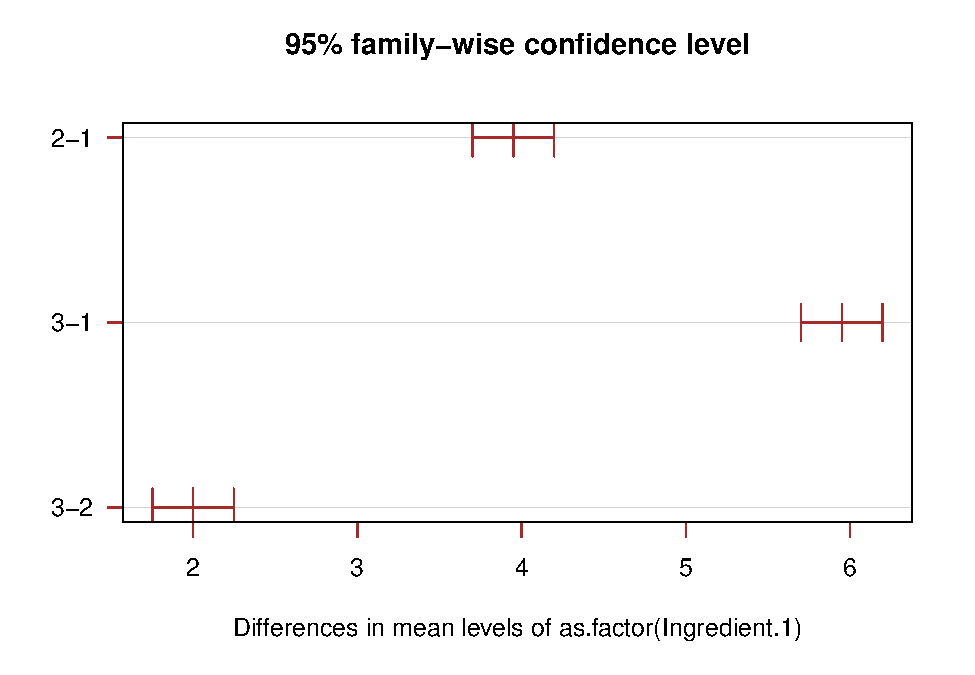
\includegraphics{STA207_bookdown_files/figure-latex/unnamed-chunk-12-1.pdf}
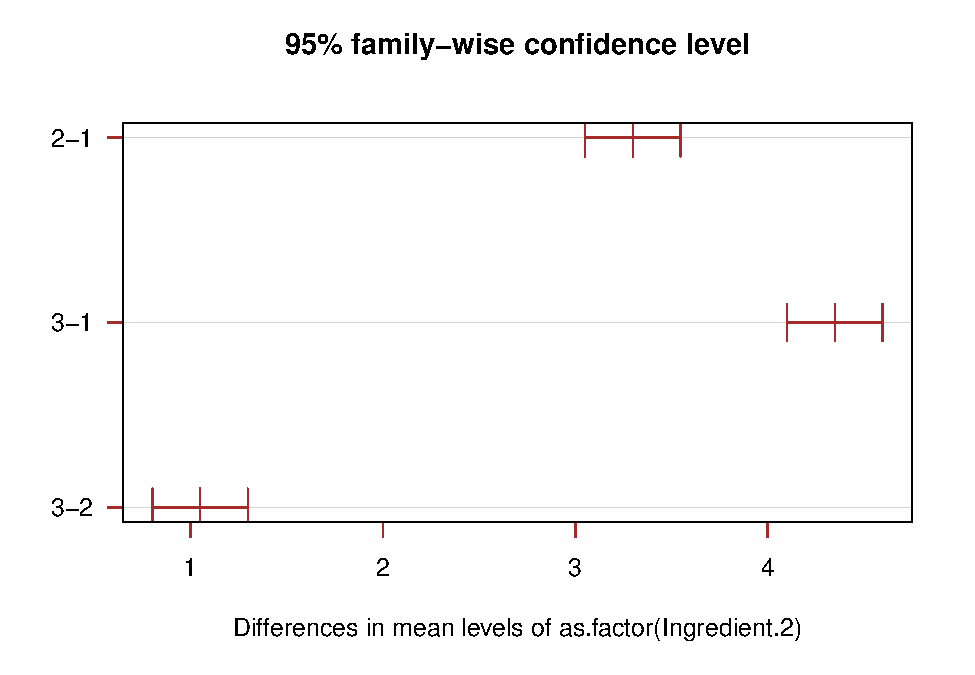
\includegraphics{STA207_bookdown_files/figure-latex/unnamed-chunk-12-2.pdf}
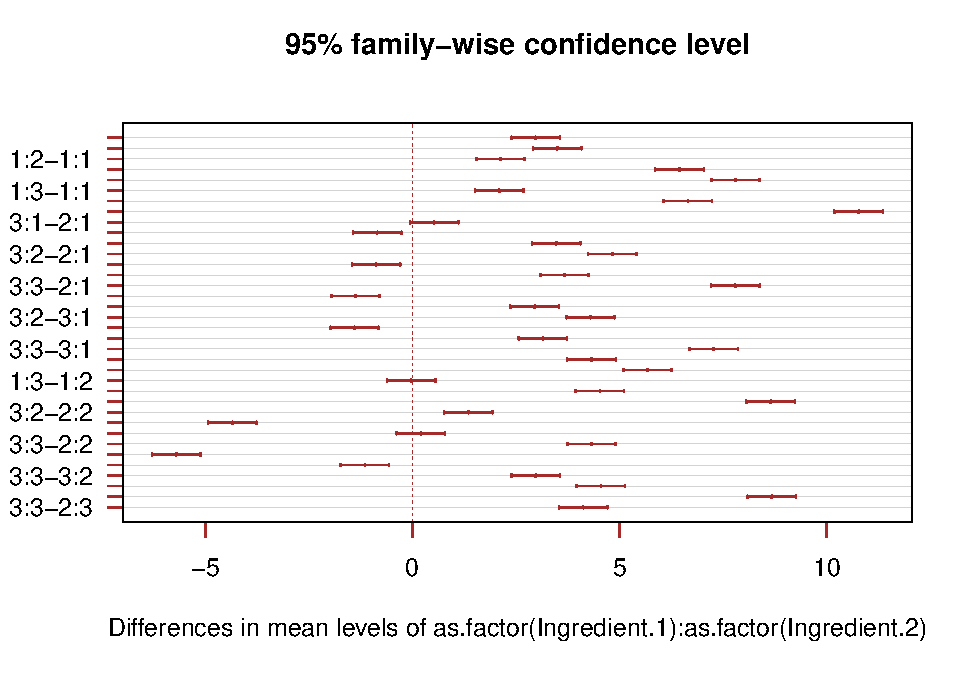
\includegraphics{STA207_bookdown_files/figure-latex/unnamed-chunk-12-3.pdf}

\begin{Shaded}
\begin{Highlighting}[]
\CommentTok{# We only need to pay attention to the differences of the two largest means}
\NormalTok{idx=}\KeywordTok{list}\NormalTok{();}
\NormalTok{idx[[}\DecValTok{1}\NormalTok{]]=Hay}\OperatorTok{$}\NormalTok{Ingredient.}\DecValTok{1}\NormalTok{;idx[[}\DecValTok{2}\NormalTok{]]=Hay}\OperatorTok{$}\NormalTok{Ingredient.}\DecValTok{2}\NormalTok{;}
\NormalTok{(}\DataTypeTok{means.comb=}\KeywordTok{tapply}\NormalTok{( Hay}\OperatorTok{$}\NormalTok{Relief, }\DataTypeTok{INDEX=}\NormalTok{idx,mean))}
\end{Highlighting}
\end{Shaded}

\begin{verbatim}
##     1    2    3
## 1 2.5  4.6  4.6
## 2 5.4  8.9  9.1
## 3 6.0 10.3 13.2
\end{verbatim}

\begin{Shaded}
\begin{Highlighting}[]
\CommentTok{# For model diagnostics, we can use the default plotting function of aov()}

\KeywordTok{plot}\NormalTok{(anova.fit)}
\end{Highlighting}
\end{Shaded}

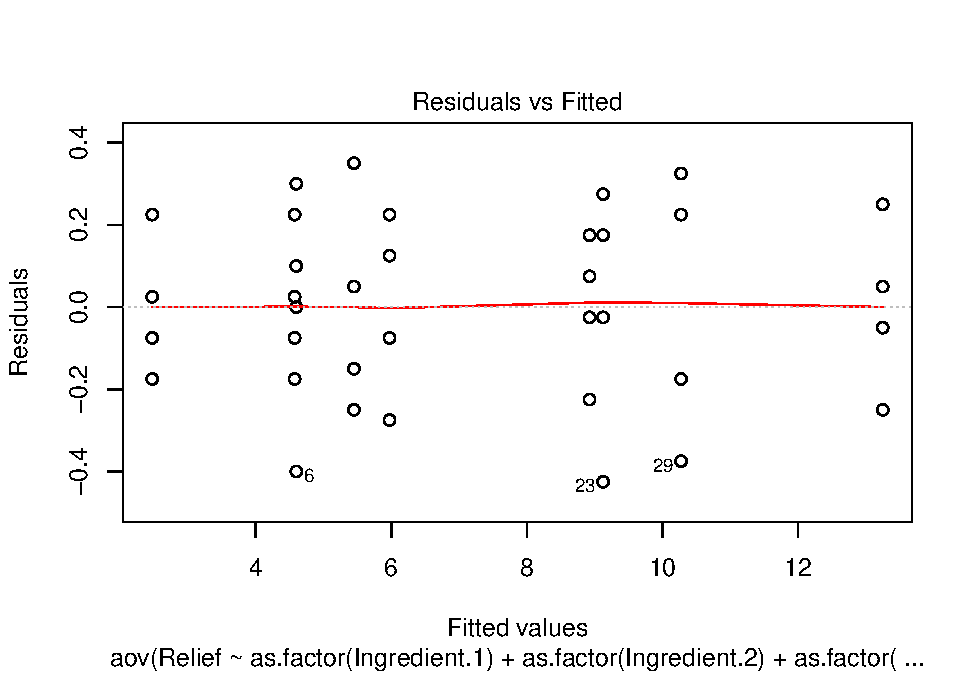
\includegraphics{STA207_bookdown_files/figure-latex/unnamed-chunk-13-1.pdf}
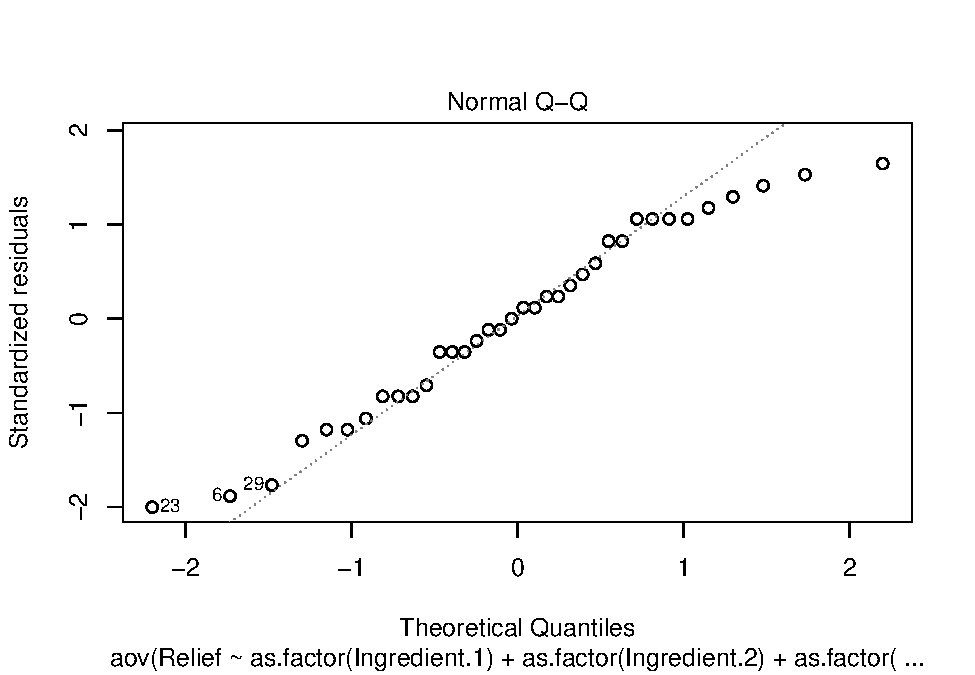
\includegraphics{STA207_bookdown_files/figure-latex/unnamed-chunk-13-2.pdf}
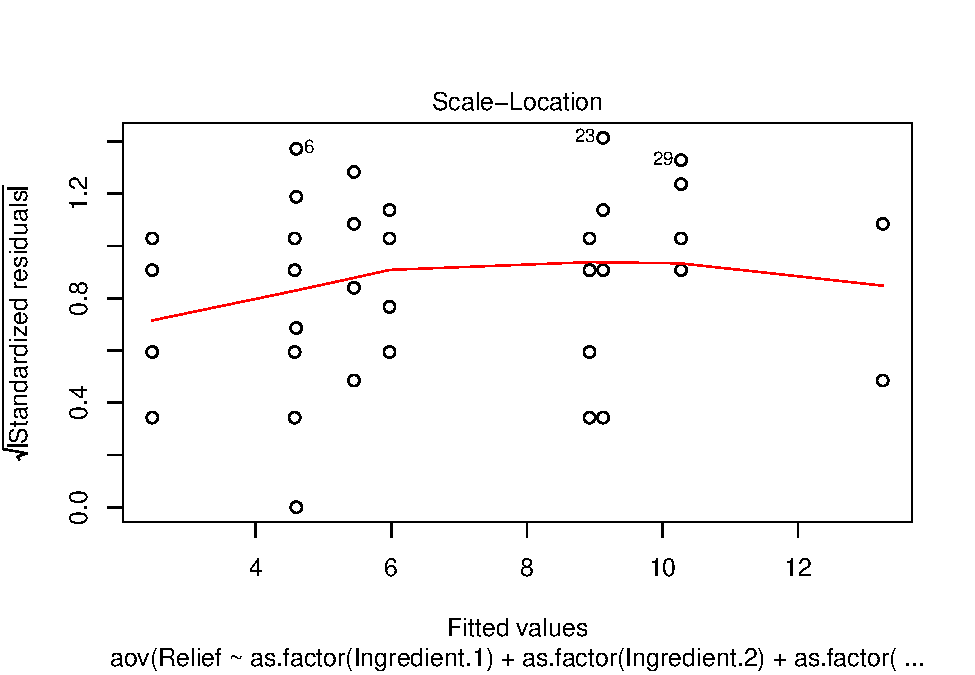
\includegraphics{STA207_bookdown_files/figure-latex/unnamed-chunk-13-3.pdf}
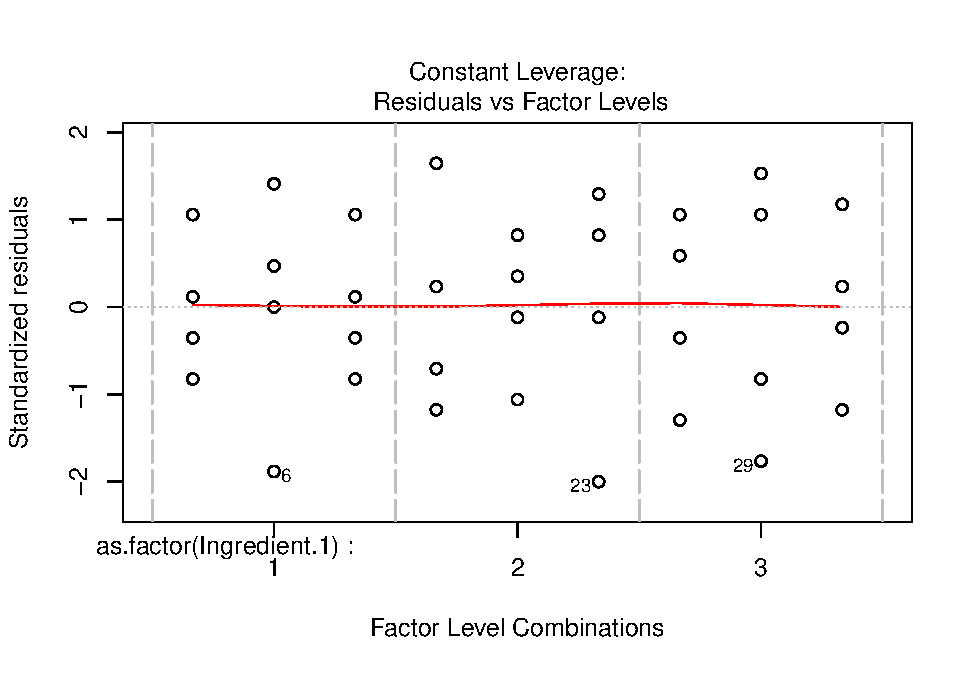
\includegraphics{STA207_bookdown_files/figure-latex/unnamed-chunk-13-4.pdf}

\subsection{Special case: one observation per
cell}\label{special-case-one-observation-per-cell}

\begin{itemize}
\tightlist
\item
  Interaction effects are no longer identifiable
\item
  Estimation and testing
\item
  Tukey's test of additivity
\end{itemize}

\subsection{Unbalanced two-way ANOVA}\label{unbalanced-two-way-anova}

\begin{itemize}
\tightlist
\item
  The model is the same as for the balanced case
\item
  Estimators for the means and variances
\item
  Hypothesis testing

  \begin{itemize}
  \tightlist
  \item
    Interaction effects
  \item
    Main effects
  \end{itemize}
\item
  Missing data in the one observation per cell case
\end{itemize}

\subsection{Analysis of stratified
experiments}\label{analysis-of-stratified-experiments}

\begin{itemize}
\tightlist
\item
  Why stratification?
\end{itemize}

We can check whether stratification is efficient on the auditor training
data.

\begin{Shaded}
\begin{Highlighting}[]
\NormalTok{Audit <-}\StringTok{ }\KeywordTok{read.csv}\NormalTok{(}\DataTypeTok{file=}\StringTok{"./data/AuditorTraining.csv"}\NormalTok{, }\DataTypeTok{header=}\OtherTok{TRUE}\NormalTok{, }\DataTypeTok{sep=}\StringTok{","}\NormalTok{)}

\CommentTok{# Or draw the interaction plot:}
\KeywordTok{interaction.plot}\NormalTok{(Audit}\OperatorTok{$}\NormalTok{Block, Audit}\OperatorTok{$}\NormalTok{Method,Audit}\OperatorTok{$}\NormalTok{Proficiency)}
\end{Highlighting}
\end{Shaded}

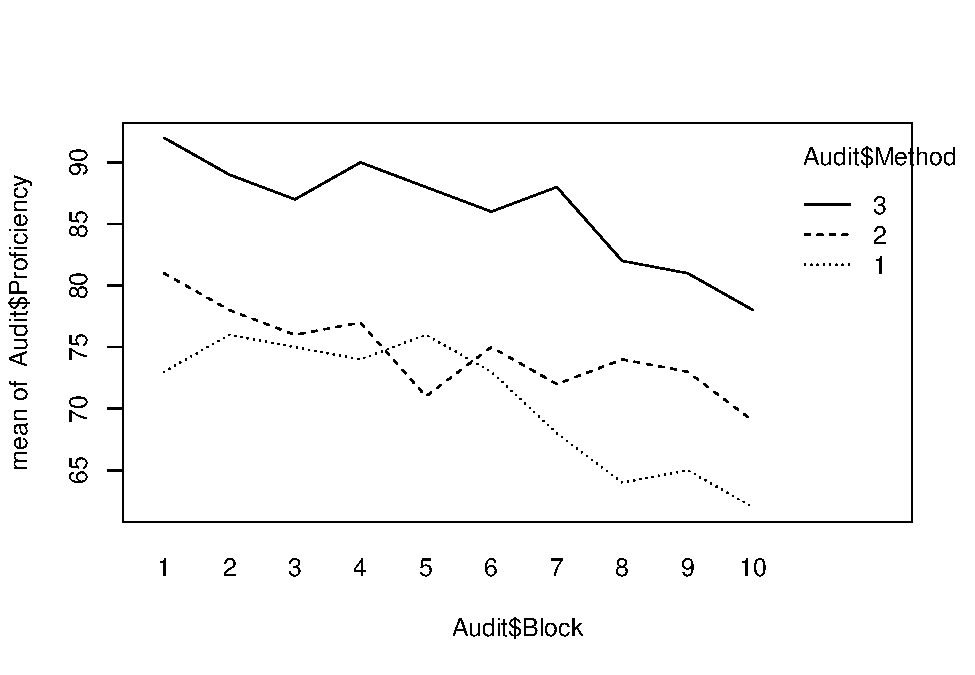
\includegraphics{STA207_bookdown_files/figure-latex/unnamed-chunk-14-1.pdf}

\begin{Shaded}
\begin{Highlighting}[]
\CommentTok{# Fit the model with blocks:}
\NormalTok{anova.block<-}\KeywordTok{aov}\NormalTok{(Proficiency}\OperatorTok{~}\KeywordTok{as.factor}\NormalTok{(Block)}\OperatorTok{+}\KeywordTok{as.factor}\NormalTok{(Method),}\DataTypeTok{data=}\NormalTok{Audit)}
\NormalTok{anova.random<-}\KeywordTok{aov}\NormalTok{(Proficiency}\OperatorTok{~}\KeywordTok{as.factor}\NormalTok{(Method),}\DataTypeTok{data=}\NormalTok{Audit)}

\NormalTok{mse.block<-}\KeywordTok{sum}\NormalTok{(anova.block}\OperatorTok{$}\NormalTok{residuals}\OperatorTok{^}\DecValTok{2}\NormalTok{)}\OperatorTok{/}\NormalTok{anova.block}\OperatorTok{$}\NormalTok{df.residual}
\NormalTok{mse.random<-}\KeywordTok{sum}\NormalTok{(anova.random}\OperatorTok{$}\NormalTok{residuals}\OperatorTok{^}\DecValTok{2}\NormalTok{)}\OperatorTok{/}\NormalTok{anova.random}\OperatorTok{$}\NormalTok{df.residual}
\NormalTok{(}\DataTypeTok{E=}\NormalTok{mse.random}\OperatorTok{/}\NormalTok{mse.block)}
\end{Highlighting}
\end{Shaded}

\begin{verbatim}
## [1] 3.2
\end{verbatim}

\section{Learning Objectives}\label{learning-objectives-2}

\begin{itemize}
\tightlist
\item
  Students are able to write down an appropriate two-way ANOVA model
  given a new dataset.
\item
  Students understand the basic properties of the various types of
  two-way ANOVA models.
\item
  Students recognize the assumptions associated with each method, and
  can find appropriate tests to verify the assumptions.
\item
  Students can implement the aforemened tasks in \texttt{R}.
\item
  Students can seek help in coding using the Internet.
\end{itemize}

\chapter{Random and Mixed Effect Models}\label{ch:nested}

(In progress)

\section{Nested design}\label{nested-design}

\begin{itemize}
\tightlist
\item
  Motivations for a nested design
\item
  Nested design with fixed factors

  \begin{itemize}
  \tightlist
  \item
    Sampling scheme
  \item
    Hypothesis testing
  \item
    Causal interpretation
  \end{itemize}
\item
  Nested design with random factors
\item
  Nested design with mixed factors

  \begin{itemize}
  \tightlist
  \item
    Repeated measures design
  \end{itemize}
\end{itemize}

\section{Random effects model}\label{random-effects-model}

\begin{itemize}
\tightlist
\item
  One-way ANOVA model with random effects
\item
  Estimation

  \begin{itemize}
  \tightlist
  \item
    Decomposition of variances
  \end{itemize}
\item
  Hypothesis testing and confidence intervals
\end{itemize}

\subsection{Mixed effects model}\label{mixed-effects-model}

\subsection{Unbalanced mixed and random effect
models}\label{unbalanced-mixed-and-random-effect-models}

\section{Learning Objectives}\label{learning-objectives-3}

\begin{itemize}
\tightlist
\item
  Students are able to write down the two-way ANOVA model with random
  effects.
\item
  Students can properly decide whether to model a factor using fixed or
  random effects.
\item
  Students recognize the key assumptions associated with the random
  effects model.
\item
  Students can implement the aforemened tasks in \texttt{R}.
\item
  Students can explore extension of random effect model from the
  Internet.
\end{itemize}

\chapter{Repeated Measures Design}\label{ch:repeated}

(In progress)

\section{Repeated measures design}\label{repeated-measures-design}

\begin{itemize}
\tightlist
\item
  Motivation for repeated measures
\item
  Sampling scheme
\item
  Estimation, hypothesis, and causal interpretation
\item
  Split plot design
\item
  Longitudinal data

  \begin{itemize}
  \tightlist
  \item
    Experiments
  \item
    Observational studies: prospective and retrospective cohort study
  \item
    Sampling scheme for observational studies
  \end{itemize}
\end{itemize}

\section{Analysis of repeated measures
designs}\label{analysis-of-repeated-measures-designs}

\subsection{Motivating data: blood
pressure}\label{motivating-data-blood-pressure}

The relationship between the dose of a drug that increases blood
pressure and the actual amount of increase in mean systolic blood
pressure was investigated in a laboratory experiment. Twelve rabbits
received in random order six different dose levels of the drug, with a
suitable time interval between each drug administration. The increase in
blood pressure was used as the response variable.

\subsection{Two-way ANOVA model}\label{two-way-anova-model}

\begin{itemize}
\tightlist
\item
  Model
\item
  Estimators
\item
  Sum of squares and mean squares
\item
  Statistical inference

  \begin{itemize}
  \tightlist
  \item
    Hypothesis testing
  \item
    Confidence intervals
  \end{itemize}
\end{itemize}

\subsection{More complicated repeated measures
design}\label{more-complicated-repeated-measures-design}

\begin{itemize}
\tightlist
\item
  Two factors with repeated measures on one factor
\item
  Two factors with repeated measures on both
\item
  Split-plot design
\end{itemize}

\subsection{Longitudinal data
analysis}\label{longitudinal-data-analysis}

We consider the rat growth data. Each rat is measured over 5 weeks. This
type of data set is called longitudinal since the observations are taken
over time. There is a covariate ``mother's weight'' (X). The idea is to
see how rat weights vary over time since birth. In another example,
logarithm of CD4 counts are listed for patients on three different
treatments over time. Goal is to investigate how CD4 counts change over
time and if age has any effect on this change. Note that in the first
example, the times at which measurement are taken are the same for all
subjects. In the second case times may be different for different
patients.

We consider several models to fit them in \texttt{R}.

\chapter{Case-control Study}\label{ch:case}

(In progress)

\section{Case-control study}\label{case-control-study}

\begin{itemize}
\tightlist
\item
  Study design
\item
  Sampling schemes
\item
  Comparisons to other studies

  \begin{itemize}
  \tightlist
  \item
    randomized experiments
  \item
    retrospective cohort studies
  \end{itemize}
\item
  Motivation for a case-control study
\item
  Estimands in a case-control study
\end{itemize}

\section{Logistic regression}\label{logistic-regression}

\begin{itemize}
\tightlist
\item
  Logistic regression models
\item
  Estimation via maximum likelihood

  \begin{itemize}
  \tightlist
  \item
    Simple case with analytic solution
  \item
    Score function
  \item
    Fisher information
  \end{itemize}
\item
  Statistical inference

  \begin{itemize}
  \tightlist
  \item
    Hypothesis testing
  \item
    Confidence intervals
  \end{itemize}
\item
  Diagnostic plots

  \begin{itemize}
  \tightlist
  \item
    Residuals
  \item
    Pearson residuals
  \end{itemize}
\end{itemize}

\section{Generalized linear model}\label{generalized-linear-model}

\begin{itemize}
\tightlist
\item
  Basics of generalized linear models
\item
  Practical use of GLM
\end{itemize}

\chapter{Observational Study}\label{ch:obs}

(Optional topic)

\chapter{Complex data}\label{ch:dim}

(Optional topic)

\chapter{Project description}\label{ch:proj}

If a statistical method is employed, you need to clearly state the model
and justify your choice.

\section{Project 1: Project STAR I}\label{project-1-project-star-i}

\subsection{Background}\label{background}

In this project, we study the dataset from a very influential randomized
experient. Tennesses Student/Teacher Achievement Ratio study (Project
STAR) was conducted in the late 1980s to evaluate the effect of class
size on test scores. This dataset has been used as a classic examples in
many textbooks and research papers. You are encouraged to read more
about the experiment design and how others analyze this dataset. This
document only provides a brief explanation of the dataset that suffices
for this course project.

The study randomly assigned students to small classes, regular classes,
and regular classes with a teacher's aide. In order to randomize
properly, schools were enrolled only if they had enough studybody to
have at least one class of each type. Once the schools were enrolled,
students were randomly assigned to the three types of classes, and one
teacher was randomly assigned to one class.

The dataset contains scaled scores for math and reading from
kindergarten to 3rd grade. We will only examine the math scores in 1st
grade in this project.

\subsection{Tasks}\label{tasks}

\begin{enumerate}
\def\labelenumi{\arabic{enumi}.}
\tightlist
\item
  Install the \texttt{AER} package and load the \texttt{STAR} dataset.\\
\item
  Explore this dataset and generate summary statistics (in forms of
  tables or plots) that you find informative, and explain them.\\
\item
  Write down a one-way ANOVA model to study the effects of class types
  on the math scaled scores. Explain your notation.
\item
  Explain why your model is appropriate for this task on this data set.
  You may want to include statistics and plots in your explanation.
\item
  Fit the model you choose in Task 3 and show your fits in the report.
\item
  Conduct model diagnostic and/or sensitivity analysis.
\item
  Test whether there is a difference in the math scaled score in 1st
  grade across students in different class types. Justify your choice of
  test.
\item
  Discuss whether you are able to make any causal statements based on
  your analysis.
\end{enumerate}

\section{Project 2: Project STAR II}\label{project-2-project-star-ii}

\subsection{Background}\label{background-1}

We will continue our study on Project STAR. In the previous project, we
examine the effects on individual students. Here we consider each
teacher as the individual unit. Moreover, we will also explore the
longitudinal feature of this dataset and the fact that randomization
happened within schools.

\subsection{Tasks}\label{tasks-1}

\begin{enumerate}
\def\labelenumi{\arabic{enumi}.}
\tightlist
\item
  Explore math scaled scores in the 1st and 2nd grades with teachers as
  the unit. Generate summary statistics (in forms of tables or plots)
  that you find informative, and explain them.
\item
  Write down a two-way ANOVA model to study the effects of class types
  on scores, with the school indicator as the other factor. Explain your
  notation.
\item
  Explain why your model is appropriate for this task on this data set.
  You may want to include statistics and plots in your explanation.
\item
  Fit the model you choose in Task 2 and show your fits in the report.
\item
  Conduct model diagnostic and/or sensitivity analysis.
\item
  Test whether there is a difference in the math scaled score in
  kindergarten across students in different class types. Justify your
  choice of test.
\item
  Discuss whether you are able to make any causal statements based on
  your analysis.
\item
  Is there any difference between the results from this analysis
  compared to the analysis from Project 1?
\end{enumerate}

\section{Project 3: US Traffic
Fatalities}\label{project-3-us-traffic-fatalities}

\subsection{Background}\label{background-2}

The National Highway Traffic Safety Administration reported that there
are 36,560 highway fatalities across US in 2018
(\href{nhtsa.gov/press-releases/roadway-fatalities-2018-fars}{link}).
Alarmed by the high traffic fatalities, you wanted to use your knowledge
and skills in statistics to explore measures that can potentially reduce
the traffic fatalities.

You found out that traffic fatalities data for 48 US states from 1982 to
1988 are available, and well-cleaned, in an \texttt{R} package
\texttt{AER}. You can see more description of the data set from the help
file of the \texttt{fatalities} dataset (e.g., using
\texttt{?Fatalities}).

You want to analyze this dataset to see if there are any of the
variables that \emph{caused} the reduction or increase of traffic
fatalities. Note that the ultimate goal is to make suggestions to policy
makers to take certain measures.

The beer tax is the tax on a case of beer, which is an available measure
of state alcohol taxes more generally. The drinking age variable is a
factor indicating whether the legal drinking age is 18, 19, or 20. The
two binary punishment variables describe the state's minimum sentencing
requirements for an initial drunk driving conviction.

Total vehicle miles traveled annually by state was obtained from the
Department of Transportation. Personal income was obtained from the US
Bureau of Economic Analysis, and the unemployment rate was obtained from
the US Bureau of Labor Statistics

\subsection{Tasks}\label{tasks-2}

\begin{enumerate}
\def\labelenumi{\arabic{enumi}.}
\tightlist
\item
  Explore this dataset and generate summary statistics (in forms of
  tables or plots) that you find crucial for your own interest, or for
  convincing the policy makers.
\item
  Consider only the data in year 1982, propose a regression model to
  study whether having a mandatory jail sentence reduce the traffic
  fatalities. In particular, you need to

  \begin{enumerate}
  \def\labelenumii{\alph{enumii}.}
  \tightlist
  \item
    define the causal effect,
  \item
    state the assumptions required, c, write down your model, d, fit the
    model with appropriate methods, e, and conduct model diagnostics
    and/or sensitivity analysis.
  \end{enumerate}
\item
  Conclude your analysis results, and interpret them. You may want to
  test a hypothesis, construct a confidence interval, or draw a
  confidence band.
\item
  Explain your analysis results to policy makers who may know little
  about statistics.
\item
  Consider the full dataset from 1982 to 1988, conduct Tasks 2 and 3.
\item
  Are there any notable differences between your analysis in Task 2 and
  Task 5? If so, explain these differences.
\end{enumerate}

\section{Project 4: Bank Marketing}\label{project-4-bank-marketing}

\subsection{Background}\label{background-3}

A Portuguese retail bank started a telemarketing campaign in 2008,
aiming to subscribe new users to a long-term deposit. Information
collected during the campaign was recorded in this data set. More
information is available on the UCI machine learning repository
(\href{https://archive.ics.uci.edu/ml/datasets/Bank+Marketing\#}{link})
and the citations therein.

You are a consultant who is hired to study the retail banking market in
Portugese. Somehow you come to know such a dataset is publicly
available. Naturally, you want to gain some insights of the market from
this dataset, before conducting an expensive survey.

\subsection{Tasks}\label{tasks-3}

\begin{enumerate}
\def\labelenumi{\arabic{enumi}.}
\tightlist
\item
  Acquire the dataset from the UCI machine learning repository
  (\href{https://archive.ics.uci.edu/ml/datasets/Bank+Marketing\#}{link}).
\item
  Pick an appropriate data set to study, and justify your decision.
\item
  Explore this dataset and generate summary statistics (in forms of
  tables or plots) that you find crucial for your clients to know.
\item
  Build a predictive model for whether a client will sign on to a
  long-term deposit. You will use logistic regression in this task.
  Specifically, you will

  \begin{enumerate}
  \def\labelenumii{\alph{enumii}.}
  \tightlist
  \item
    write down a property logistic regression model,
  \item
    fit the model,
  \item
    evaluate the performance of the fitted model,
  \item
    and conduct model diagnostic and/or sensitivity analysis.
  \end{enumerate}
\item
  Build another predictive model using random forest, and compare its
  performance compared to the logistic regression.
\item
  Explain the possible gap in the performances to your supervisor, who
  knows statistics quite well and only believes in data and
  mathematics.\\
\item
  Test whether having a house loan will increase the likelihood of a
  client to sign up for a long-term deposit. (Hint: you don't need to
  use the same model as in Task 4.)
\item
  Explain your conclusion from the test to your clients who know little
  about statistics.
\end{enumerate}

\bibliography{book.bib,packages.bib}


\end{document}
